\documentclass[11pt,a4 paper,title page]{article}
\usepackage[utf8]{inputenc}
\usepackage{natbib}
\usepackage{graphicx}
\usepackage{float}
\usepackage{lineno}
\usepackage[colorlinks = true,
            linkcolor = teal,
            urlcolor  = teal,
            citecolor = black,
            anchorcolor = blue]{hyperref}
  \usepackage{wrapfig}
  \setlength{\pdfpagewidth}{9in} \setlength{\pdfpageheight}{12in}
\usepackage{amsmath}
\usepackage{ragged2e}
\usepackage{hyperref}
\usepackage{epstopdf}

 \title{\textbf{Mini Project :Population Growth}}
\author{\large\textbf{Liying Huang}\\
\textbf{supervisor: Dr Samraat Pawar }\\
\textbf{Faculty of Natural Sciences,},\\
\textbf{Department of Life Sciences (Silwood Park)},\\
\textbf{s.pawar@imperial.ac.uk}}
\date{\Large{\textbf{March 2020},\\
\textbf{WORD COUNT: 2563}}}
\begin{document}
\maketitle
\linenumbers 
 \section{Introduction}
  Natural populations are composed of individuals with diverse phenotypes that show differences in their demographic parameters and intra- and inter-species interaction(\cite{bolnick2011intraspecific}. Fluctuations in individual population abundance may play a key role in ecosystem dynamics and emerging functional characteristics. When the abundance is low and the resources are not limited, the population abundance will increase exponentially, which is the Malthus principle (\cite{malthus1992malthus}. The Malthusian principle also points out that when resources become limited, population growth will gradually slow down and eventually stop. At the same time, there may be a period of time before population growth really starts, which is called the lag phase. The data used in this simulation was collected through laboratory experiments around the world, ensuring the sample size of this experiment. In this report, I used different models to simulate the growth process of population abundance, and made comparison and analysis to obtain the most suitable model for the growth process of experimental samples.

  \section{Background}
  This project using 4 model, the logistic equation model, the modified Gompertz model, The Baranyi model and The Buchanan model. 

    \subsection{The logistic equation model}
    This model is the simplest mathematical models that we can use the phenomenological quadratic and cubic polynomial models. In general, if the quantitative characteristics of objective things are: at time t is small, things grow exponentially, and when t increases, the growth rate gradually decreases and gets closer and closer to a certain value (that is, bearing capacity Nmax), such problems can be solved by the Logistic equation (\cite{weisstein2003logistic}.
\begin{figure}[H]
\centering
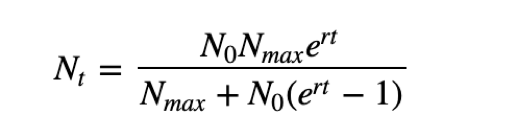
\includegraphics[height=1in,angle=360]{../picture/figure1.png}
\end{figure}
\hfill\break
Nt is population size at time t
\hfill\break
N0 is initial cell culture (Population) density
\hfill\break
Nmax is maximum population density, called carrying capacity
\hfill\break
t is time that is parameters in the sample data
\hfill\break
r is maximum growth rate 


    \subsection{The modified Gompertz model}
    
    This model is often used in the literature to simulate bacterial growth.It is a function of the sigmoid colon and describes the slowest growth at the beginning and end of a given time period. This is the most widely accepted detailed convention on population growth.The right-hand or future value asymptote(A) of the function is closer to the curve than the left Side or lower asymptotes (\cite{zwietering1990modeling}.
\begin{figure}[H]
\centering
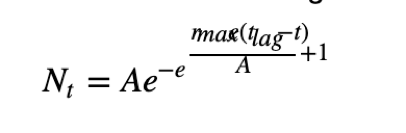
\includegraphics[height=1in,angle=360]{../picture/figure2.png}
\end{figure}
\hfill\break
Nt is population size at time t
\hfill\break
N0 is initial cell culture (Population) density
\hfill\break
Nmax is maximum population density, called carrying capacity
\hfill\break
t is time that is parameters in the sample data
\hfill\break
rmax is maximum growth rate 
\hfill\break
tlag is the x-axis intercept to this tangent, means duration of the delay before the population starts growing exponentially
\hfill\break
A=ln(Nmax/N0), is the asymptote.


    \subsection{The Baranyi model}
    Four kinds of common survival curves are fitted with Baranyi model: linear curve, hysteresis curve, trailing curve and sigmoid curve.This model adds a new dimensionless parameter h0 which represents the initial physiological state of the cells. For the prediction performance, the Baranyi model was better and more robust than the modified Gompertz equation (\cite{xiong1999comparison}.
\begin{figure}[H]
\centering
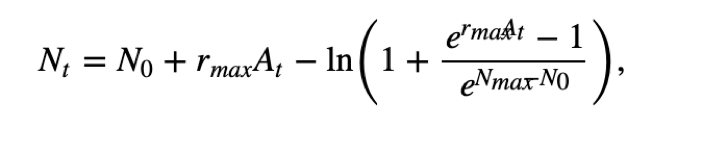
\includegraphics[height=1in,angle=360]{../picture/figure3.png}
\end{figure}
    \hfill\break
    where:
    \begin{figure}[H]
\centering
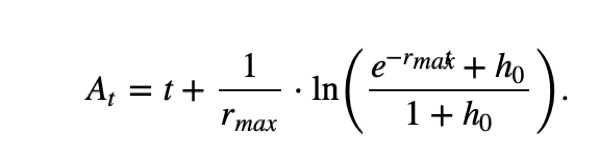
\includegraphics[height=1in,angle=360]{../picture/figure4.png}
\end{figure}

\begin{figure}[H]
\centering
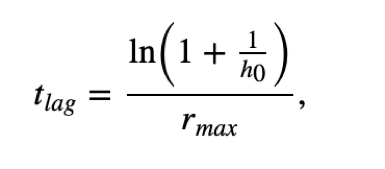
\includegraphics[height=1in,angle=360]{../picture/figure5.png}
\end{figure}
    \hfill\break
Nt is population size at time t
    \hfill\break
N0 is initial cell culture (Population) density
    \hfill\break
Nmax is maximum population density, called carrying capacity
    \hfill\break
t is time that is parameters in the sample data
    \hfill\break
rmax is maximum growth rate 
    \hfill\break
tlag is the x-axis intercept to this tangent, means duration of the delay
    \hfill\break
before the population starts growing exponentially

    \subsection{The Buchanan model}
    This model can be called as three-phase logistic model. Three-phase is an Initial Phase, Intermediate Phase, and Final Phase. The initial stage means that t≤tlag, relatively stable, or flat over time. The Intermediate Phase refers to tlag < t < tmax. After the initial stage, the growth rate may change. If the initial population is much smaller than the carrying capacity, the population will increase rapidly. If the initial population abundance is much larger than the carrying capacity, the population will decrease rapidly. If the initial population abundance approaches the capacity, the population abundance will tend to be stable. Final phase means tlag ≤ t, when the population abundence reach the carrying capacity. At this point, the population abundance will be stable, unless the carrying capacity changes(\cite{lopez2004statistical}.
\begin{figure}[H]
\centering
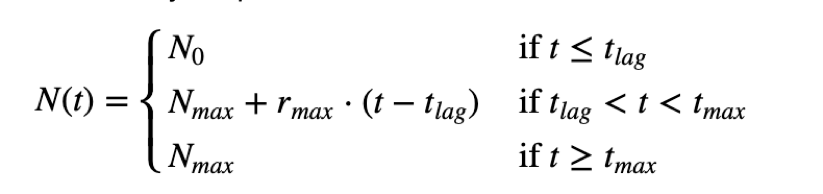
\includegraphics[height=1in,angle=360]{../picture/figure6.png}
\end{figure}
    \hfill\break
    Nt is population size at time t
    \hfill\break
N0 is initial cell culture (Population) density
\hfill\break
Nmax is maximum population density, called carrying capacity
\hfill\break
t is time that is parameters in the sample data
\hfill\break
rmax is maximum growth rate 
\hfill\break
tlag is the x-axis intercept to this tangent, means duration of the delay before the population starts growing exponentially

  \section{methods and data}

    \subsection{Computing tools}
In this project, I use three scripting language to write this project. Python, R and Script. Python is used to filter data from sample data and find some parameter that I will use in the next program. R is used to simulate the model and perform the nls operation (fit the model), while generating pictures and final data. Script is used to run all programs, reducing the time required to manually run the programs and increasing the efficiency of the project. In python, I call a lot of packages to reduce some unnecessary runtime and memory usage. I write two python program. The first program is used to filter data. For this purpose, I called pandas, seaborn, math as a package. Pandas used to be create new DataFrame to store data.
\begin{figure}[H]
\centering
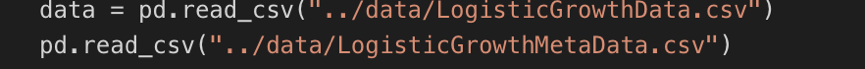
\includegraphics[width=.8\textwidth]{../picture/figure7.png}
\end{figure}
\hfill\break
I prefer to use DataFrames to organize data over lists. Using DataFrames to organize time faster, reduce runtime and memory data.
\hfill\break
\hfill\break
Seaborn used to plot.
\begin{figure}[H]
\centering

\includegraphics[width=.8\textwidth]{../picture/figure8.png}
\end{figure}
\hfill\break
In this project, using it will plot the abundance of the population over time. But this picture is only used for the parameter reference is not needed at the end, so comment out in the code
\hfill\break
\hfill\break
Math used to calculate ln (NMAX / N0). In python, math.log() means return the natural logarithm of x.
\begin{figure}[H]
\centering
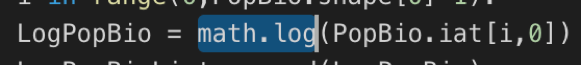
\includegraphics[width=.8\textwidth]{../picture/figure9.png}
\end{figure}
\hfill\break
The second program is used to find some parameter that I will use in the next program. For this purpose, I just called pandas. Using DataFrame to store data that I will use in the next program.
\begin{figure}[H]
\centering
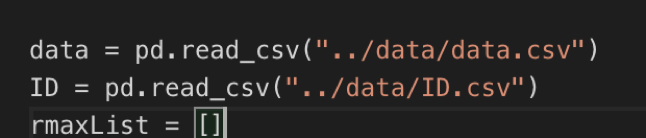
\includegraphics[width=.8\textwidth]{../picture/figure10.png}
\end{figure}
\hfill\break
In r file, I called repr, ggplot2, nls.multstart as a package. Repr used to change default plot size.
\begin{figure}[H]
\centering
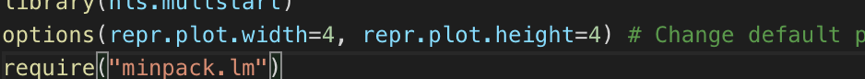
\includegraphics[width=.8\textwidth]{../picture/figure11.png}
\end{figure}
\hfill\break
ggplot2 used to plot. In this project, using it can plot the abundance of the population over time and model and sample data matching graph.
\begin{figure}[H]
\centering
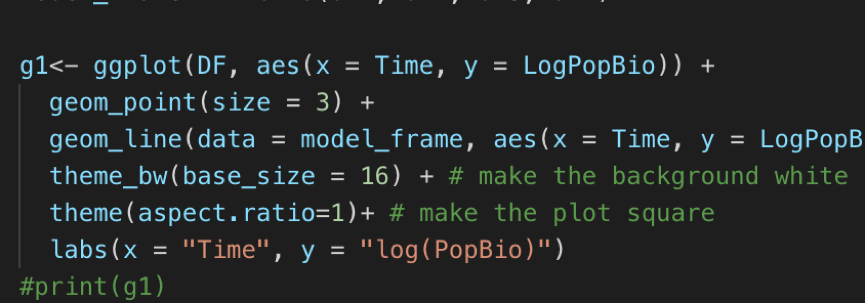
\includegraphics[width=.8\textwidth]{../picture/figure12.png}
\end{figure}
\hfill\break
nls.multstart used to NLLS fitting method. Using it to match the sample data to the four models respectively.
\begin{figure}[H]
\centering
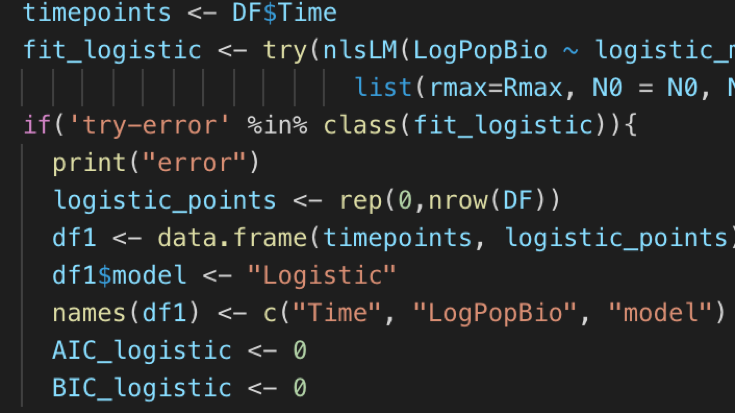
\includegraphics[width=.8\textwidth]{../picture/figure13.png}
\end{figure}
\hfill\break    
In this part, also using “try-error” method. This part will described in ‘method’ section.

    
    
    
    \subsection{Data}
    In this project, all data comes from research institutes around the world, ensuring that the amount of sample data is large enough. The sample data set is called LogisticGrowthData.CSV. It contains measurements of change in biomass or number of cells of microbes over time. Meanwhile, we will use the other data set is called LogisticGrowthMetaData.CSV. This contains a detailed description of each parameter.
Using panda.DataFrame to read these data set to our program. When we filter the data, all the filtered data is written into a new CSV, called data.CSV. The ID name corresponding to the filtered data is written to another CSV file, called ID.CSV. In all the following processes, we only use data.CSV and ID.CSV to process the data.

    \subsection{Method}
The propose of this project is compare the selected sample data with the population growth calculated by the model and to obtain the model that most conforms to the sample data. 
    \hfill\break
    \subsubsection{Process Data}
    For this purpose, we first set a unique ID for the sample data to group the sample data. In this project, I chose to evaluate the uniqueness of all parameters and make the parameter values part of the ID rather than unique. Therefore, the final ID is data.Species + data.Temp.map (str) + data.Medium +  data.Citation + data.Rep.map ( str). The role of map is to convert int to string, because in the id naming process, only parameters with type of string can be accepted. After grouping the sample data, we got 305 sets of data. Next, according to the parameters to be used, rmax, n0, nmax, tlag, and A, we extract each group with a total number of 5 or more into a single data group, and gather the corresponding ID names to build a data set. Next, we need to find the parameters use in the mathematical formula. The used parameters are n0, nmax, rmax, tlag and a. Among them, rmax refers to the maximum slope. In order to find the maximum slope, we take the simplest approach, (K = y1-y2 / x1-x2). First we set the first point as the starting point, and then use the first and second points to find the slope. After that we  use a for loop to find the slope between each two points, and finally get the maximum slope. Find the value of k while recording the x and y values, and get the value of b by y = kx + b. n0 is the minimum value in the data, nmax is the maximum value in the data, tlag is the value of x when y = n0, and A = ln (nmax / n0). After all the parameters of the first data group were found, the for loop was going to be used to find the parameters of the next data group, and the parameters obtained were combined with the parameters of the previous data group to form a new data frame. Finally, the generated data frames are written to a CSV file(LIST.CSV).
    \hfill\break
    \subsubsection{Model fitting}
    When we have processed all the data, we use R for model fitting. Read the LIST.CSV file and data.CSV file into the DataFrame, and use the subset to find the data corresponding to the same id. Next, build the model and get the parameters needed for the model. Use the NLLS fitting method to fit the model and actual data. The NLLS fitting method is used to fit the model and the actual data, the COEF value of the obtained model is extracted as a data frame, and calculated AIC and BIC. In the NLLS fitting method, some models can not be matched. Use the try-catch method to avoid errors. Finally, import the results from the previous step and print the model. Visually identify bad fits and determine whether to further optimize previous NLLS fit scripts. Meanwhile, AIC and BIC were imported to analyze the fitting results of the model and summarize the most suitable model.

    
    
  \section{Results}
  The propose of this project is to compare the selected sample data with the population growth calculated by the model, and to obtain the model that most conforms to the sample data. In this project, python, r, and script. For loop, if, try-catch, NLLS, DataFrame and other methods are used. The result contains 288 images and a CSV file, which contains AIC and BIC. The following uses some fitting models to illustrate the results.
  \hfill\break
  \subsection{Logistic Model}
  The data used in this case is id Chryseobacterium.balustinum-5-TSB-Bae, YM, Zheng, L., Hyun, JE, Jung, KS, Heu, S. and Lee, SY, 2014. Growth characteristics and biofilm formation of various spoilage bacteria isolated from fresh produce. Journal of food science, 79 (10), pp.M2072-M2080.-1, rmax = 0.000344284, n0 = -4.752591912, nmax = -1.254736278, AIC-gompertz= 29.93912607, AIC-logistic= -100.4740036, BIC-gompertz= 35.26794411, BIC-logistic= -95.14518554
\begin{figure}[H]
\centering
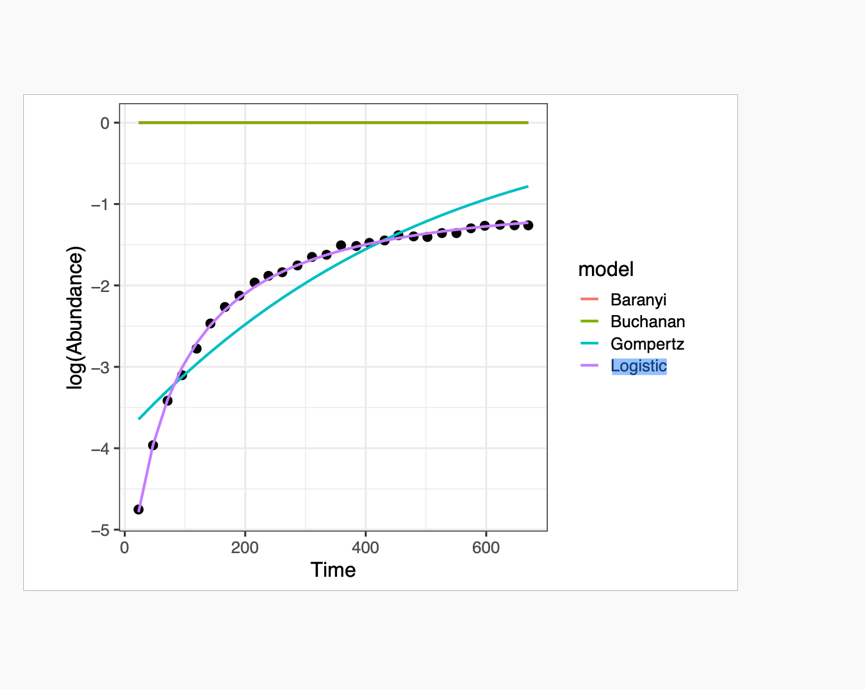
\includegraphics[width=.8\textwidth]{../picture/figure14.png}
\end{figure}
  \hfill\break
This figure shows that the Logistic model is the most suitable model. Baranyi model and Buchanan are not suitable for this data set. The curve of logistic model is generally J-shaped. As can be seen from this figure, it conforms to this special feature. When t grows from small to large, the population abundance keeps increasing. However, when the population abundance reaches a certain value, it reaches a stable state with the increase of t. From the characteristics of the logical model, if the quantitative characteristics of objective things are as follows: when time t is very small, things increase exponentially; when t increases, the growth rate gradually decreases and gets closer and closer to a certain value (that is, bearing capacity Nmax), the logical model is most suitable for this data set.
 \subsection{Gompertz Model}
  The data used in this case is id Lactobacillus sakei-30-MRS broth-Silva, A.P.R.D., Longhi, D.A., Dalcanton, F. and Arago, G.M.F.D., 2018. Modelling the growth of lactic acid bacteria at different temperatures. Brazilian Archives of Biology and Technology, 61.-1, rmax = 0.920853841, n0 = 8.817495339, nmax = 13.23583879, AIC-gompertz= 75.9798774, AIC-logistic= 45.20044445, BIC-gompertz= 77.5714585, BIC-logistic= 46.79202554

\begin{figure}[H]
\centering
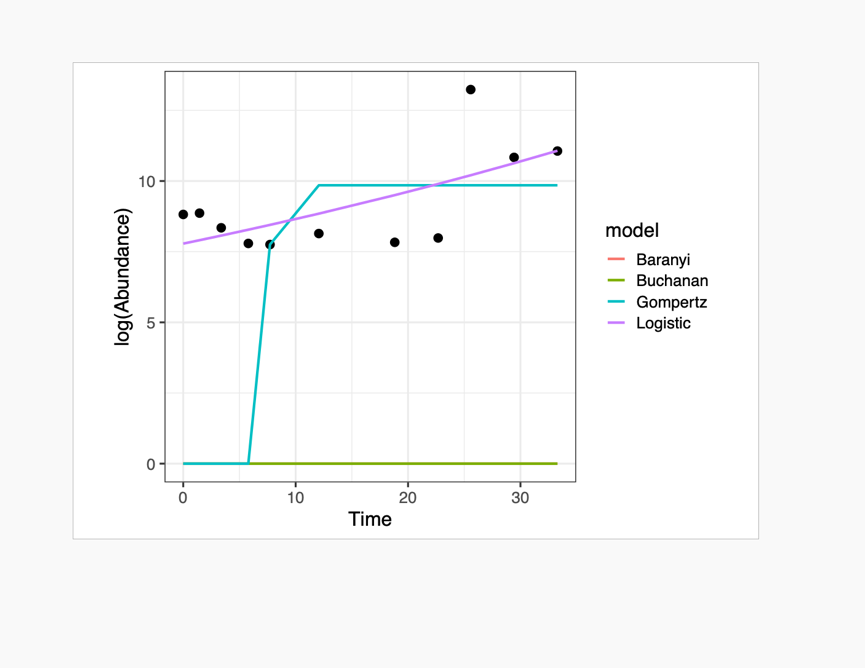
\includegraphics[width=.8\textwidth]{../picture/figure15.png}
\end{figure}
  \hfill\break
This figure shows that the Gompertz model is the most suitable model. Baranyi model and Buchanan are not suitable for this data set. The logistic model curve is generally s-shaped. As can be seen from this figure, it conforms to this special feature. When t starts to increase, the growth rate of population abundance slightly slower, and the growth rate of population abundance is accelerated in the middle period, and is slower in the later period. The Gompertz model is best suited to this data set in terms of the characteristics of a logical model that grows slowest at the beginning and end of a given time period.

 \subsection{Baranyi model}
The data used in this case is id Clavibacter.michiganensis-5-TSB-Bae, Y.M., Zheng, L., Hyun, J.E., Jung, K.S., Heu, S. and Lee, S.Y., 2014. Growth characteristics and biofilm formation of various spoilage bacteria isolated from fresh produce. Journal of food science, 79(10), pp.M2072-M2080.-1, rmax = 0.015869066, n0 = -1.437433323, nmax = -0.931062049, AIC-gompertz= 64.31968967,AIC-logistic= 60.76109259,AIC-baranyi= 55.28514297, AIC-buchanan= 66.32887698,BIC-gompertz= 69.64850771,BIC-logistic= 66.08991063, BIC-baranyi= 61.94616552, BIC-buchanan= 66.32887698
\begin{figure}[H]
\centering
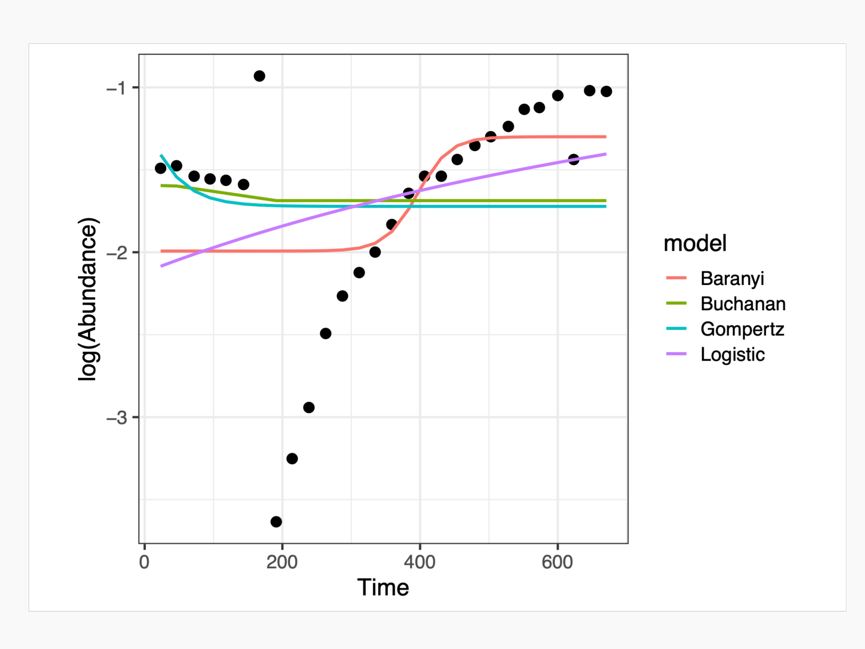
\includegraphics[width=.8\textwidth]{../picture/figure16.png}
\end{figure}
  \hfill\break
This figure shows that the Baranyi model is the most suitable model. The curves of barani model are generally linear, with hysteresis phase, trailing phase and s-shaped curve. As can be seen from this figure, it conforms to this special feature. When t starts to increase, the population abundance is already at a high level, indicating that the cells have an initial physiological state (h0). According to the characteristics of the logical model, a new dimensionless parameter h0 is added to represent the initial physiological state of the cell. Therefore, the Baranyi model is best suited for this data set.

 \subsection{Buchanan model}
The data used in this case is id Enterobacter.sp.-5-TSB-Bae, Y.M., Zheng, L., Hyun, J.E., Jung, K.S., Heu, S. and Lee, S.Y., 2014. Growth characteristics and biofilm formation of various spoilage bacteria isolated from fresh produce. Journal of food science, 79(10), pp.M2072-M2080.-1, rmax = 7.50E-05, n0 = -0.865921996, nmax = -0.541427051, AIC-gompertz= 30.20418465, AIC-logistic= 23.08963106, AIC-baranyi= 34.07912787, AIC-buchanan= 16.8633038,BIC-gompertz= 35.53300269,BIC-logistic= 28.4184491, BIC-baranyi= 40.74015042, BIC-buchanan= 16.8633038

\begin{figure}[H]
\centering
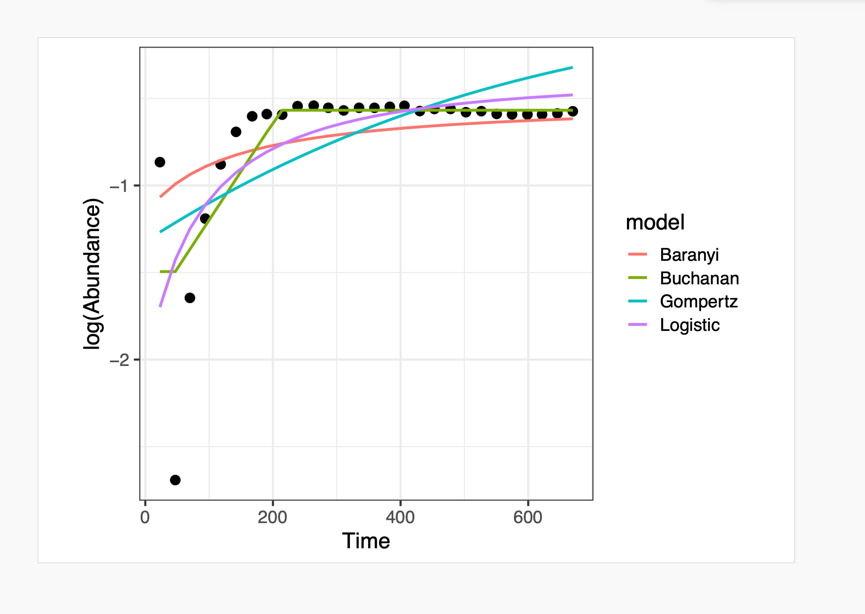
\includegraphics[width=.8\textwidth]{../picture/figure17.png}
\end{figure}
  \hfill\break
This figure shows that the Buchanan model is the most suitable model. The curve of Buchanan model is generally three-phase, and the three phases are the Initial phase, the Intermediate phase, and the Final phase. As can be seen from this figure, it conforms to this special feature. When t starts to increase, the population abundance is is relatively stable. Over time, the initial population was less than the carrying capacity, and the population abundance increased rapidly. As the population abundance approaches the carrying capacity, the population abundance remains stable.
From the characteristics of the logical model, Initial phase means t $\leq$ tlag, and is relatively stable or flat over time. Intermediate Phase means tlag <t < tmax. After the initial phase, growth rates may change. If the initial population is much smaller than the carrying capacity, the population will increase rapidly.If the initial population abundance is much greater than the carrying capacity, the population population will decrease rapidly. If the initial population abundance is close to the volume, the population abundance tends to be stable. Final phase means tlag $\leq$ t when the population abundance reach the carrying capacity. At this point, the population abundance will be stable, unless the carrying capacity changes (\cite{lopez2004statistical}. Therefore, the Buchanan model is most suitable for this data set.


  \section{Discussion}
This project verified the match between the three models and the data, but not all the data can be 100 percent matched. The problem should be that the data filter is not carefully classified.

  \bibliographystyle{plain}
  \bibliography{ReportBiblio}
\end{document}
